%%% LaTeX Template: Two column article
%%%
%%% Source: http://www.howtotex.com/
%%% Feel free to distribute this template, but please keep to referal to http://www.howtotex.com/ here.
%%% Date: February 2011

%%% Preamble
\documentclass[	DIV=calc,%
paper=a4,%
fontsize=12pt,%
onecolumn]{scrartcl}	 					% KOMA-article class
\usepackage{multicol}							%Texto em duas colunas
\usepackage{lipsum}													% Package to create dummy text
\usepackage[brazil]{babel}										% English language/hyphenation
\usepackage[protrusion=true,expansion=true]{microtype}				% Better typography
\usepackage{amsmath,amsfonts,amsthm}					% Math packages
\usepackage[pdftex]{graphicx}									% Enable pdflatex
\usepackage[svgnames]{xcolor}									% Enabling colors by their 'svgnames'
\usepackage[hang, small,labelfont=bf,up,textfont=it,up]{caption}	% Custom captions under/above floats
\usepackage{epstopdf}												% Converts .eps to .pdf
\usepackage{subfig}													% Subfigures
\usepackage{booktabs}												% Nicer tables
\usepackage{fix-cm}													% Custom fontsizes
\usepackage[utf8]{inputenc}
\usepackage[top=2.5cm, bottom=2.5cm, left=2.5cm, right=2.5cm]{geometry}
\usepackage[ddmmyyyy]{datetime}
\addto\captionsenglish{%
	\renewcommand\tablename{Tabela}
	\renewcommand\figurename{Figura}
} 



%%% Custom sectioning (sectsty package)
\usepackage{sectsty}													% Custom sectioning (see below)
\allsectionsfont{%															% Change font of al section commands
	\usefont{OT1}{phv}{b}{n}%										% bch-b-n: CharterBT-Bold font
}

\sectionfont{%																% Change font of \section command
	\usefont{OT1}{phv}{b}{n}%										% bch-b-n: CharterBT-Bold font
}



%%% Headers and footers
\usepackage{fancyhdr}												% Needed to define custom headers/footers
\pagestyle{fancy}														% Enabling the custom headers/footers
\usepackage{lastpage}	

% Header (empty)
\lhead{}
\chead{}
\rhead{}

\lfoot{\footnotesize \texttt{Cabeamento estruturado} \textbullet ~Juushin SA}


\cfoot{}
\rfoot{\footnotesize página \thepage\ de \pageref{LastPage}}	% "Page 1 of 2"
\renewcommand{\headrulewidth}{0.0pt}
\renewcommand{\footrulewidth}{0.4pt}



\usepackage{lettrine}
\newcommand{\initial}[1]{%
	\lettrine[lines=3,lhang=0.3,nindent=0em]{
		\color{DarkGoldenrod}
		{\textsf{#1}}}{}}



\usepackage{titling}															% For custom titles

\newcommand{\HorRule}{\color{DarkGoldenrod}%			% Creating a horizontal rule
	\rule{\linewidth}{1pt}%
}

\pretitle{\vspace{-30pt} \begin{flushleft} \HorRule 
		\fontsize{50}{50} \usefont{OT1}{phv}{b}{n} \color{DarkRed} \selectfont 
	}
	
	
	
	\title{Projeto de cabeamento estruturado para Juushin SA}					
	
	
	
	\posttitle{\par\end{flushleft}\vskip 0.5em}

\preauthor{\begin{flushleft}
		\large \lineskip 0.5em \usefont{OT1}{phv}{b}{sl} \color{DarkRed}}
	\author{Fernando Rocha }  	% Author name goes here
	
	
	\postauthor{\footnotesize \usefont{OT1}{phv}{m}{sl} \color{Black} 
		\\Universidade Tecnológica Federal do Paraná - Câmpus Cornélio Procópio 								% Institution of author
		\par\end{flushleft}\HorRule}

\date{}																				% No date




%%% Begin document
\begin{document}
	\maketitle
	\thispagestyle{fancy} 	
	\thispagestyle{empty}		% Enabling the custom headers/footers for the first page 
	
	\initial{E}\textbf{ste projeto tem como propósito apresentar uma estrutura de cabeamento para uma empresa fictícia, consolidando assim o conhecimento adquirido na disciplina de cabeamento estruturado.}
	
	
	\begin{figure}
		\centering
		
\includegraphics{utfpr}
	\end{figure}
	
	\vspace{2cm}
	\centerline{\textit{\textbf{\today}}}
	
	\clearpage
	\renewcommand*\listfigurename{Lista de figuras}
	\listoffigures
	
	\renewcommand*\listtablename{Lista de tabelas}
	\listoftables
	
	
	
	
	\clearpage
	\renewcommand{\contentsname}{Sumário}
	\tableofcontents
	\clearpage
	
	
	\section{Introdução}
	A Juushin SA é uma empresa que atua no área de serviços e conta, atualmente, com um quadro de 25 pessoas, sendo 9 que atuam na sede da empresa; 3 equipes de 5 pessoas, mais 1 Supervisor de equipe que atuam fora da sede. Atualmente a empresa está mudando sua sede para um novo prédio, portanto todo cabeamento será configurado a partir deste projeto.
	
	\subsection{Benefícios}
	
	O planejamento de um sistema de cabeamento traz consideráveis benefícios às empresas que o adotam, dentre eles:
	\begin{itemize}
		\item Unifica a estrutura de dados, voz e vídeo reduzindo custos com manutenção e necessidade de atualização.
		\item Menor propensão a falhas, interrupções e interferências.
		\item Uma estrutura centralizada torna as alterações, que por ventura precisem ser feitas, mais rápidas e eficientes.
		\item Diminui drasticamente a inatividade do sistema, pois o diagnóstico de problemas é mais fácil que em uma rede não estruturada.
		\item O cabeamento estruturado tem maior durabilidade, pois sofre menos manipulação e tem melhor acondicinamento. 
	\end{itemize}
	\subsection{Organizações Envolvidas}
	\begin{table}[h!] % coloque h! para forcar a posicao
		\centering
		\caption{Organizações}
		\label{tab1} %com este label vc faz referencia no texto
		\begin{tabular}{|l|l|l|l|l|l|}
			\hline
			\multicolumn{1}{|c|}{\textbf{Empresa}} & 
			\multicolumn{1}{c|}{\textbf{Serviço}} & 
			\multicolumn{1}{c|}{\textbf{Responsável}} \\ \hline
			Copel Telecom  & Provedor de Internet          & Mévio \\ \hline		
			BH Construtora & Piso e Instalação das calhas  & Caio\\ \hline
			VyperNET       & montagem Racks e cabos        & Tício \\ \hline
			Certfik       & Certificação do Cabeamento     & Plinio \\ \hline
		\end{tabular}
	\end{table}
	
	
	
	\section{Estado atual}
	Hoje, a rede da empresa encontra-se na seguinte situação:
	\begin{itemize}
		\item 1 Switch 24 portas HP 1420-24G-2SFP, 2 Switches HP 1420-8G JH329A, 500m de cabos cat5e e 1 roteador Wireless D-Link DIR-615 N .
		\item As principais reclamações dos usuários são as quedas constantes e lentidão da conexão e a demora para impressão de documentos. Aproveitando a construção da nova sede, os diretores optaram por fazer um projeto de cabeamento estruturado.
	Após análise da rede foi possível encontrar vários pontos que possam estar ocasionando os problemas relatados pelos usuários, entre eles:
		\item Cabos de rede e elétricos acondicionados juntos;
		\item Cabos de rede dobrados ou retorcidos;
		\item Cabos de rede sem identificação;		
		\item Conectores não padronizados;
		\item Switch com portas danificadas;
	\end{itemize}
	
	\section{Requisitos}
	A nova estrutura de rede deve eliminar os problemas atuais de conexão e ainda:
	\begin{itemize}
		\item Padronizar toda a estrutura de rede.
		\item Identificar os cabos.
		\item Separar o cabeamento de rede do cabeamento elétrico.
		\item Acondicionar adequadamente os equipamentos de rede.
		\item Atender demanda atual de rede e futuras expansões.				
	\end{itemize}	
	
	\section{Usuários e Aplicativos}
	Atualmente a empresa tem como usuários seus 25 colaboradores mais os clientes que fazem uso da rede sem fio. Com a crescente demanda por serviços este número pode aumentar nos próximos anos, por isso é importante que o projeto preveja uma possível expansão da rede atual.
	
	\begin{multicols}{2}
	\subsection{Usuários}
	\begin{itemize}
		\item Diretores: 3;
		\item Atendentes: 2;
		\item Administrativo: 4;
		\item Membros das Equipes: 15;
		\item Clientes: até 20;
	\end{itemize}
	\subsection{Aplicativos}
	\begin{itemize}
		\item Sistema ERP: 9;
		\item Pacote Office: 9;
		\item Sistema de Vendas: 4;
		\item Software Contábil: 1;
	\end{itemize}
	\end{multicols}{2}
	\section{Estrutura predial existente}
	Como a empresa está transferindo sua sede para um novo prédio, não convém falar sobre a estrutura predial existente. Este documento discorrerá apenas sobre a nova estrutura.
	%inicio dos comandos para criar uma nova pagina A3 horizontal
	\clearpage
	\KOMAoptions{paper=a3, paper=landscape, DIV=20}
	\recalctypearea
	
	\begin{figure}
		%	\centering
		\noindent\makebox[\textwidth][c]{
			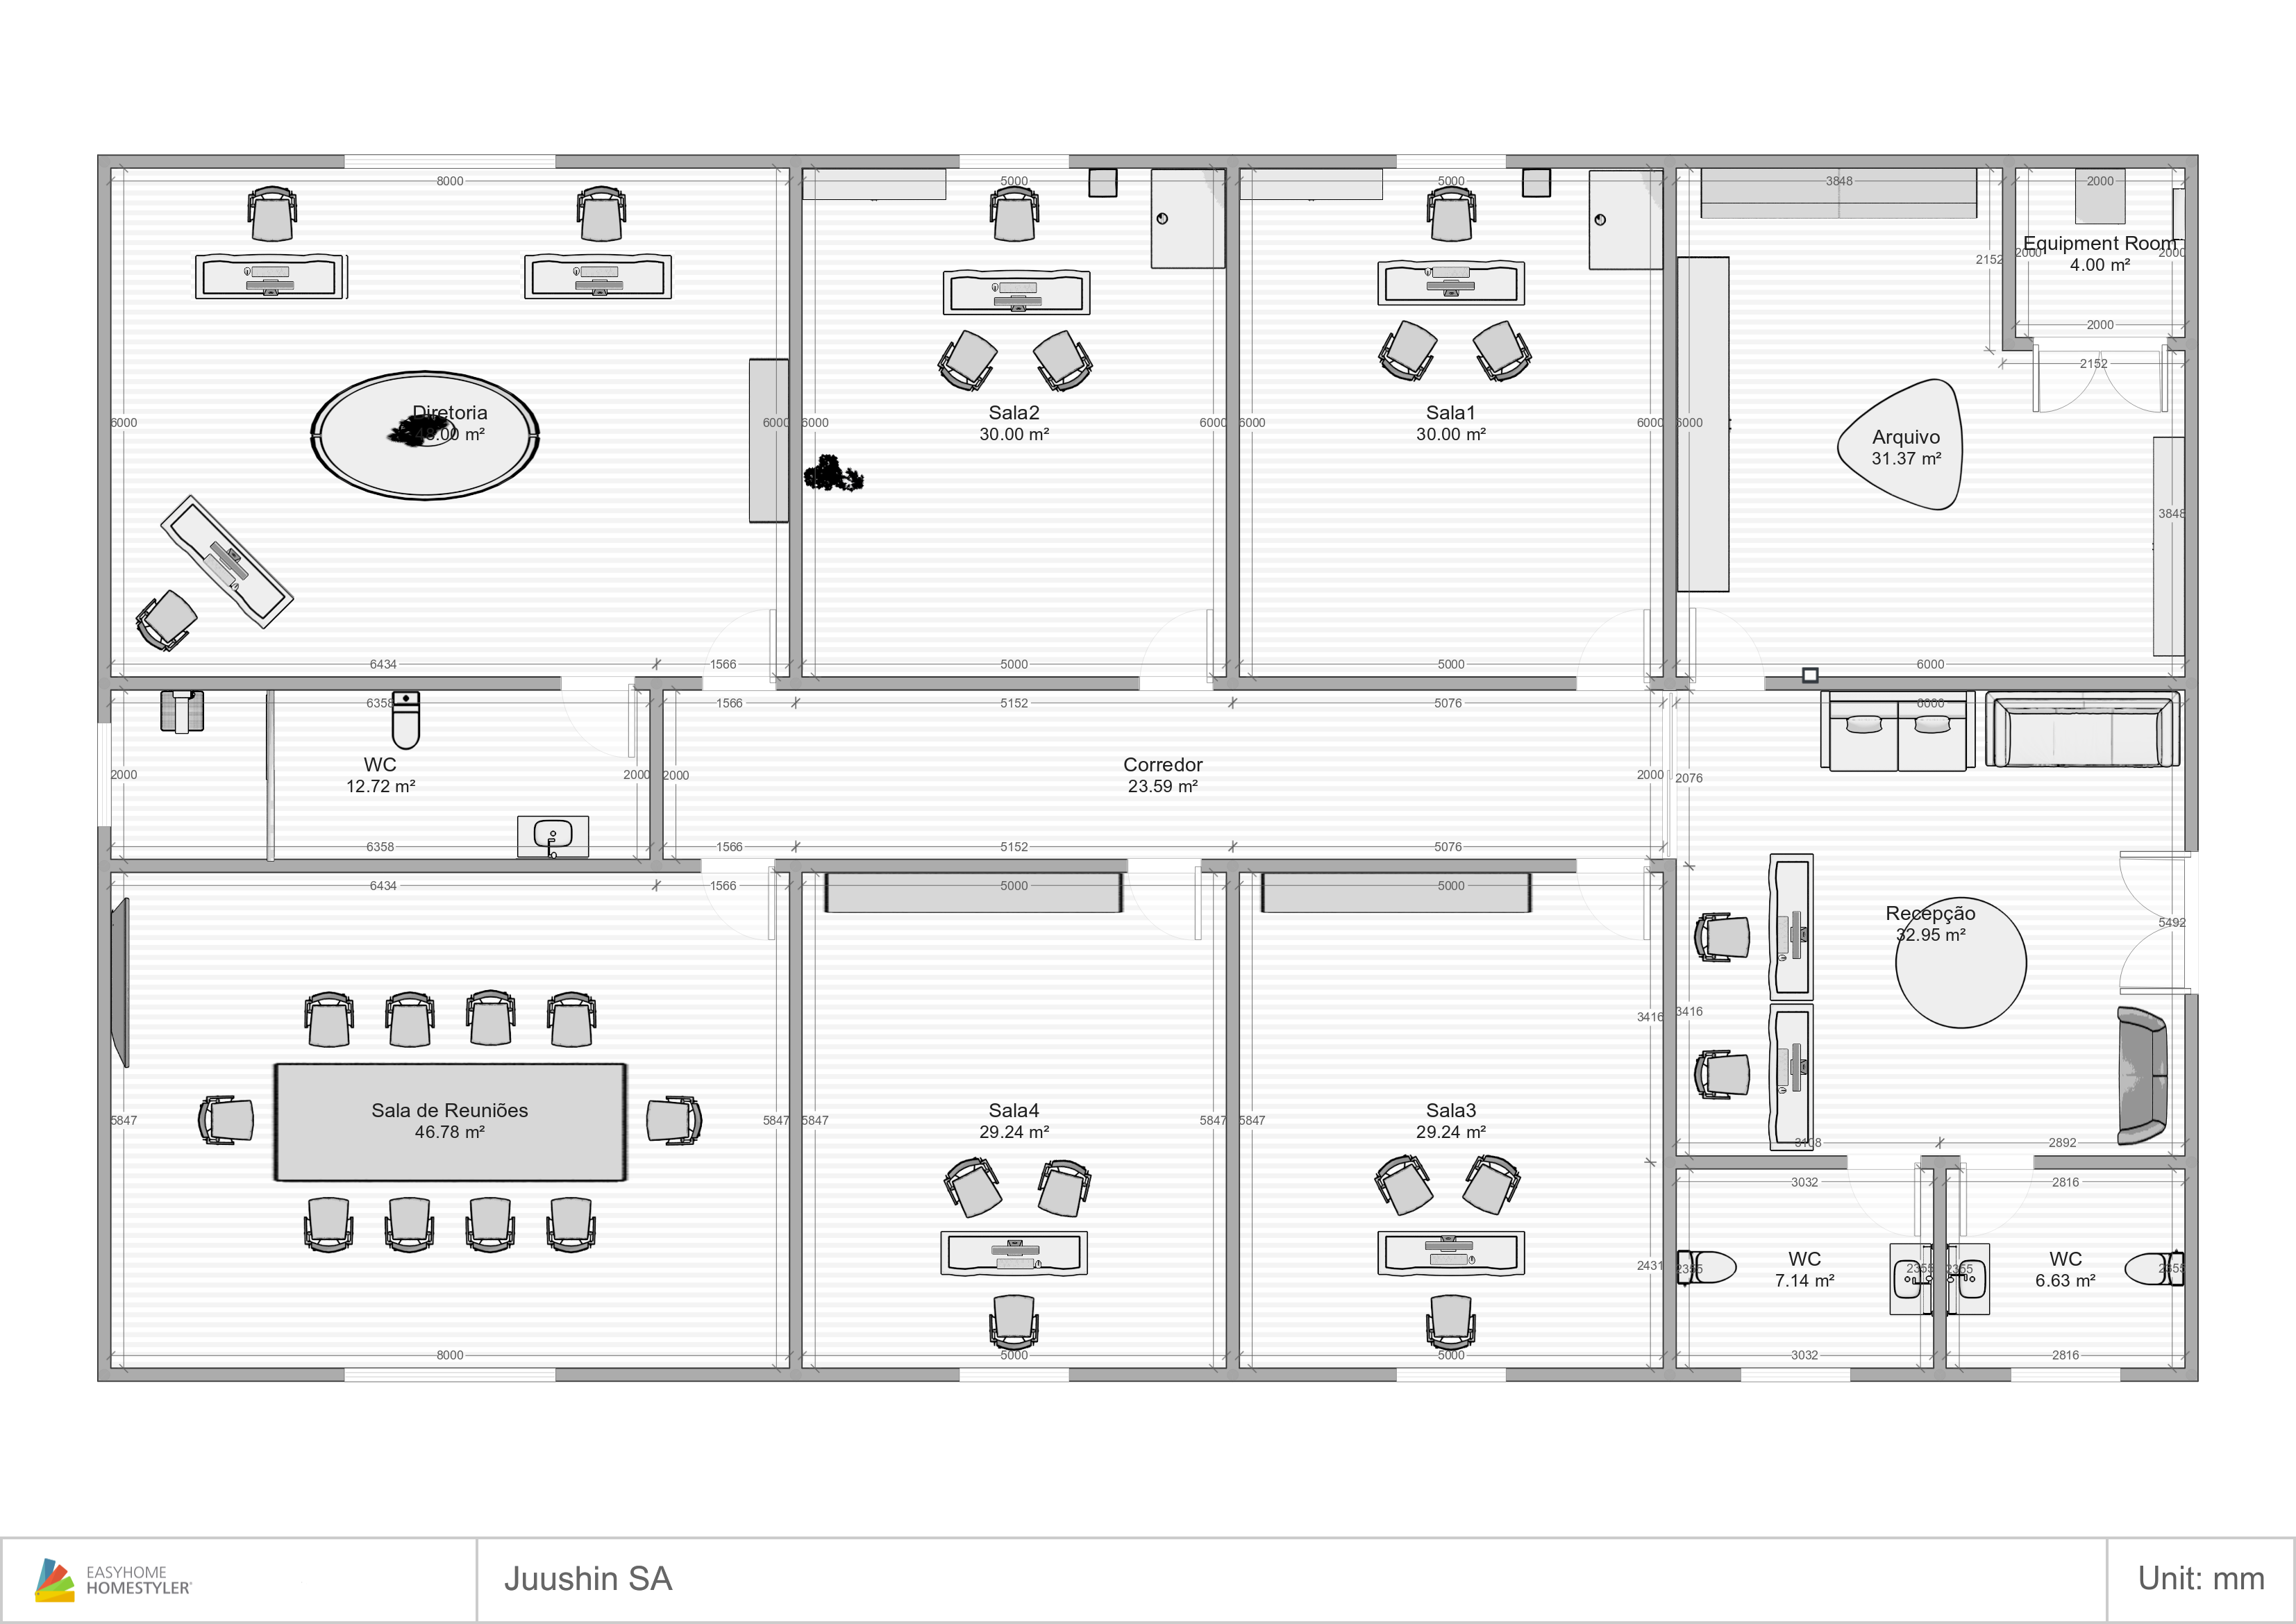
\includegraphics[width=\textwidth]{fig1}
		}
		\caption{Planta física}
		\label{fig1}
	\end{figure}
	
	%Retornar ao formato A4
	\clearpage
	\KOMAoptions{paper=a4, paper=portrait, DIV=calc}
	\recalctypearea
	%-- reinicio em A4 
	
	\section{Planta Lógica - Elementos estruturados}
	
	\subsection{Topologia}
	
		A planta da nova sede conta com uma sala de recepção com $ 32,95m^{2}  $ e 4 pontos de rede com espaçamento de 2 metros; quatro salas administrativas com aprox. $ 30m^{2}  $ e 5 pontos de rede com espaçamento de 2 metros; uma sala de diretores com $ 48m^{2}  $ e 6 pontos de rede com espaçamento de 2 metros; uma sala para reuniões com $ 46,78m^{2}  $ e 8 pontos de rede com espaçamento de 2 metros;  3 banheiros e uma sala de arquivos com $ 31,37m^{2}  $ e 4 pontos de rede com espaçamento de 2 metros, onde se encontra a sala de equipamentos.
		
		\begin{figure}[h]
			\centering
			
			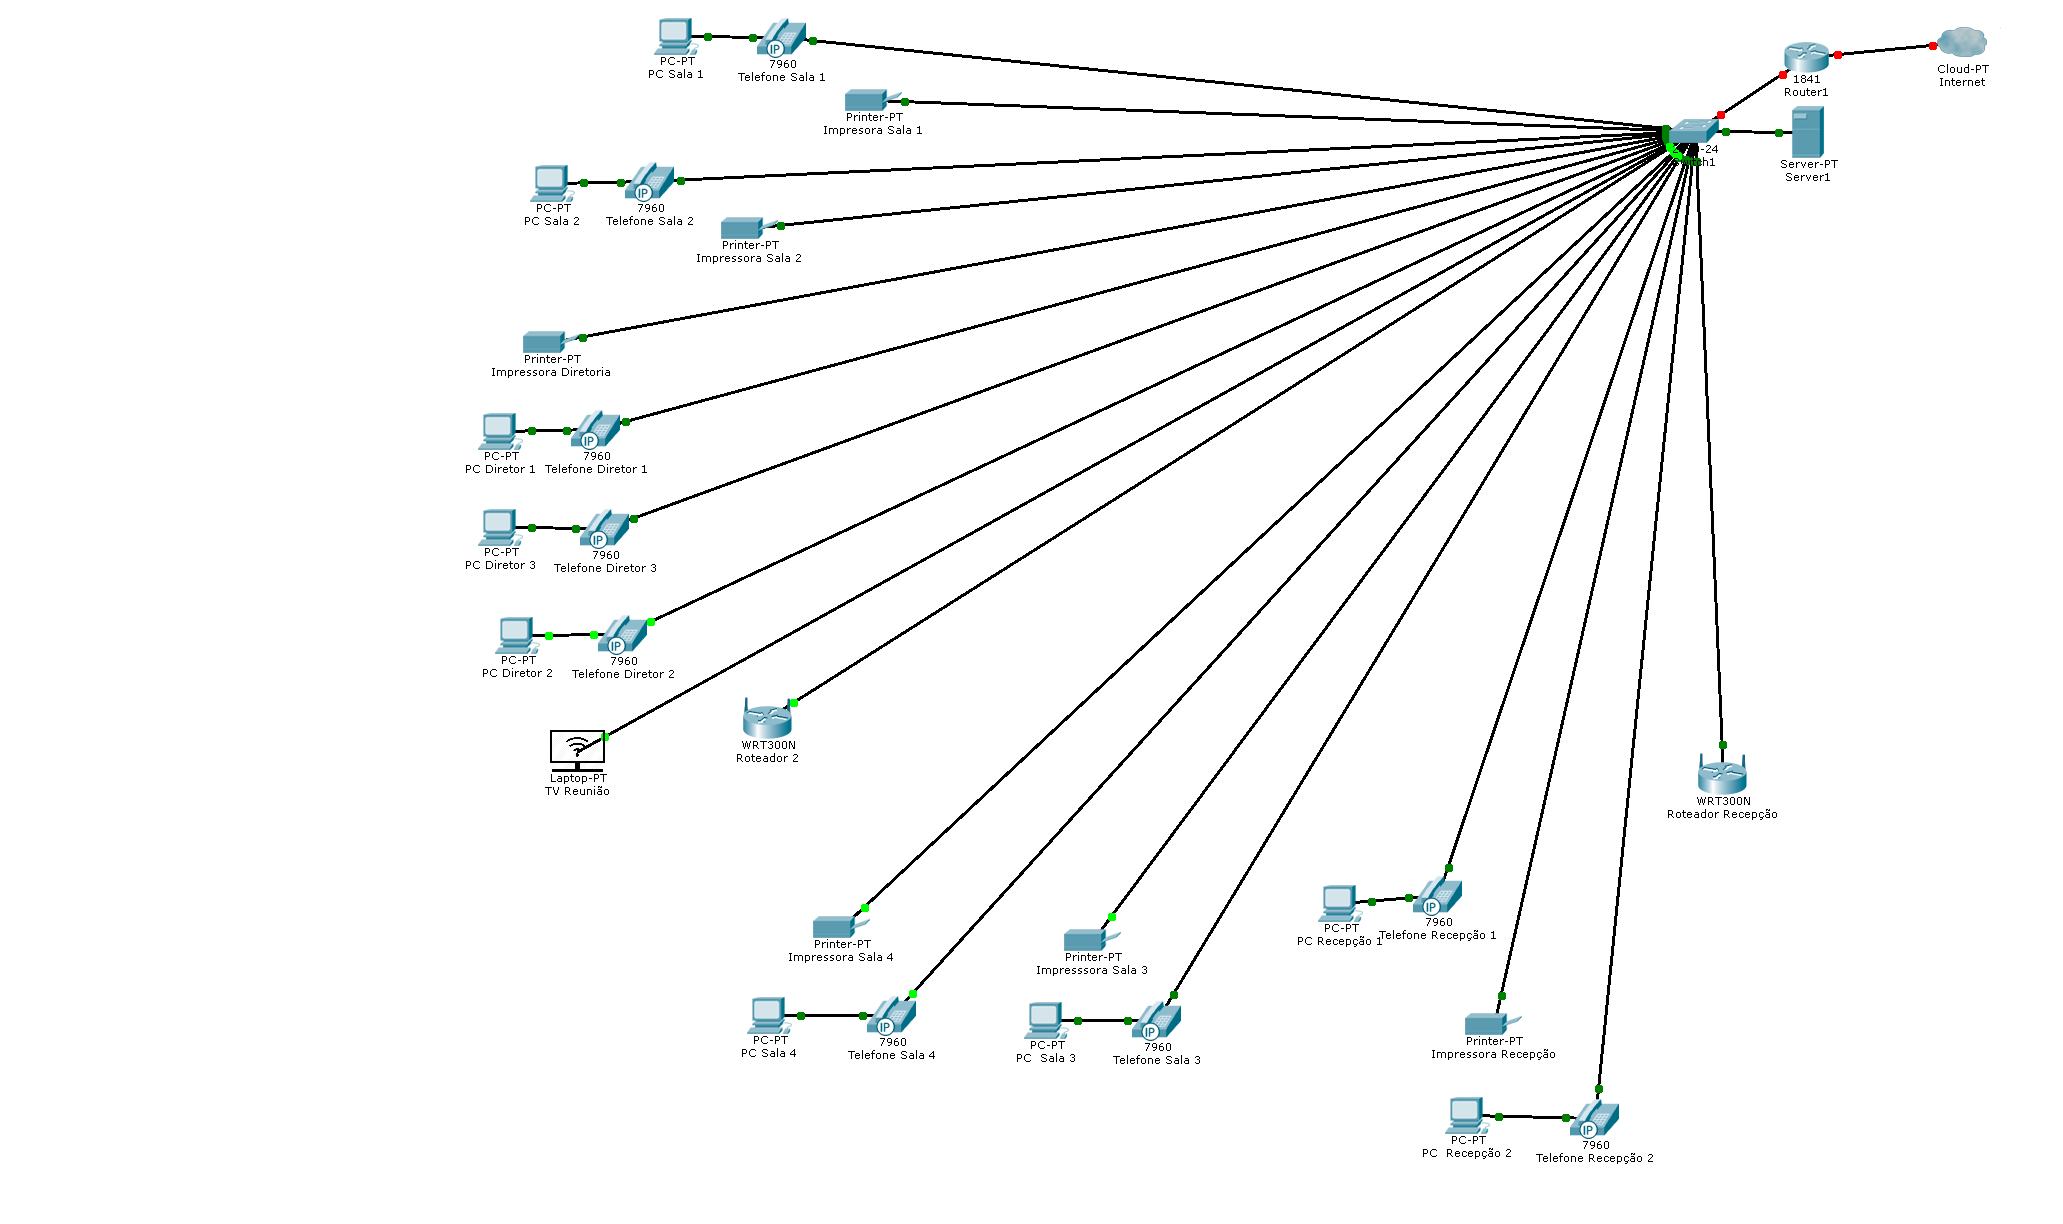
\includegraphics[width=\textwidth]{fig2}
			\caption{Planta Lógica}
			\label{fig2}
		\end{figure}
	
	\subsection{Encaminhamento}
	Os cabos seguirão em eletrocalhas sob o piso elevado e sairão por eletrodutos até as tomadas, localizadas a 0,45m acima do piso.A Eletrocalha "A", identificada no projeto com a cor azul, conterá o cabeamento da sala 1, sala 2 e sala da diretoria, totalizando 14 cabos.
	A eletrocalha "B", identificada no projeto com a cor vermelha, conterá o cabeamento da sala 3, sala 4 e sala de reuniões.	A eletrocalha "C", identificada no projeto com a cor verde, conterá o cabeamento da sala de arquivos, recepção, sala 3, sala 4 e sala de reuniões. 
	
	
	%inicio dos comandos para criar uma nova pagina A3 horizontal
	\clearpage
	\KOMAoptions{paper=a3, paper=landscape, DIV=20}
	\recalctypearea
	
	\begin{figure}
		%	\centering
		\noindent\makebox[\textwidth][c]{
			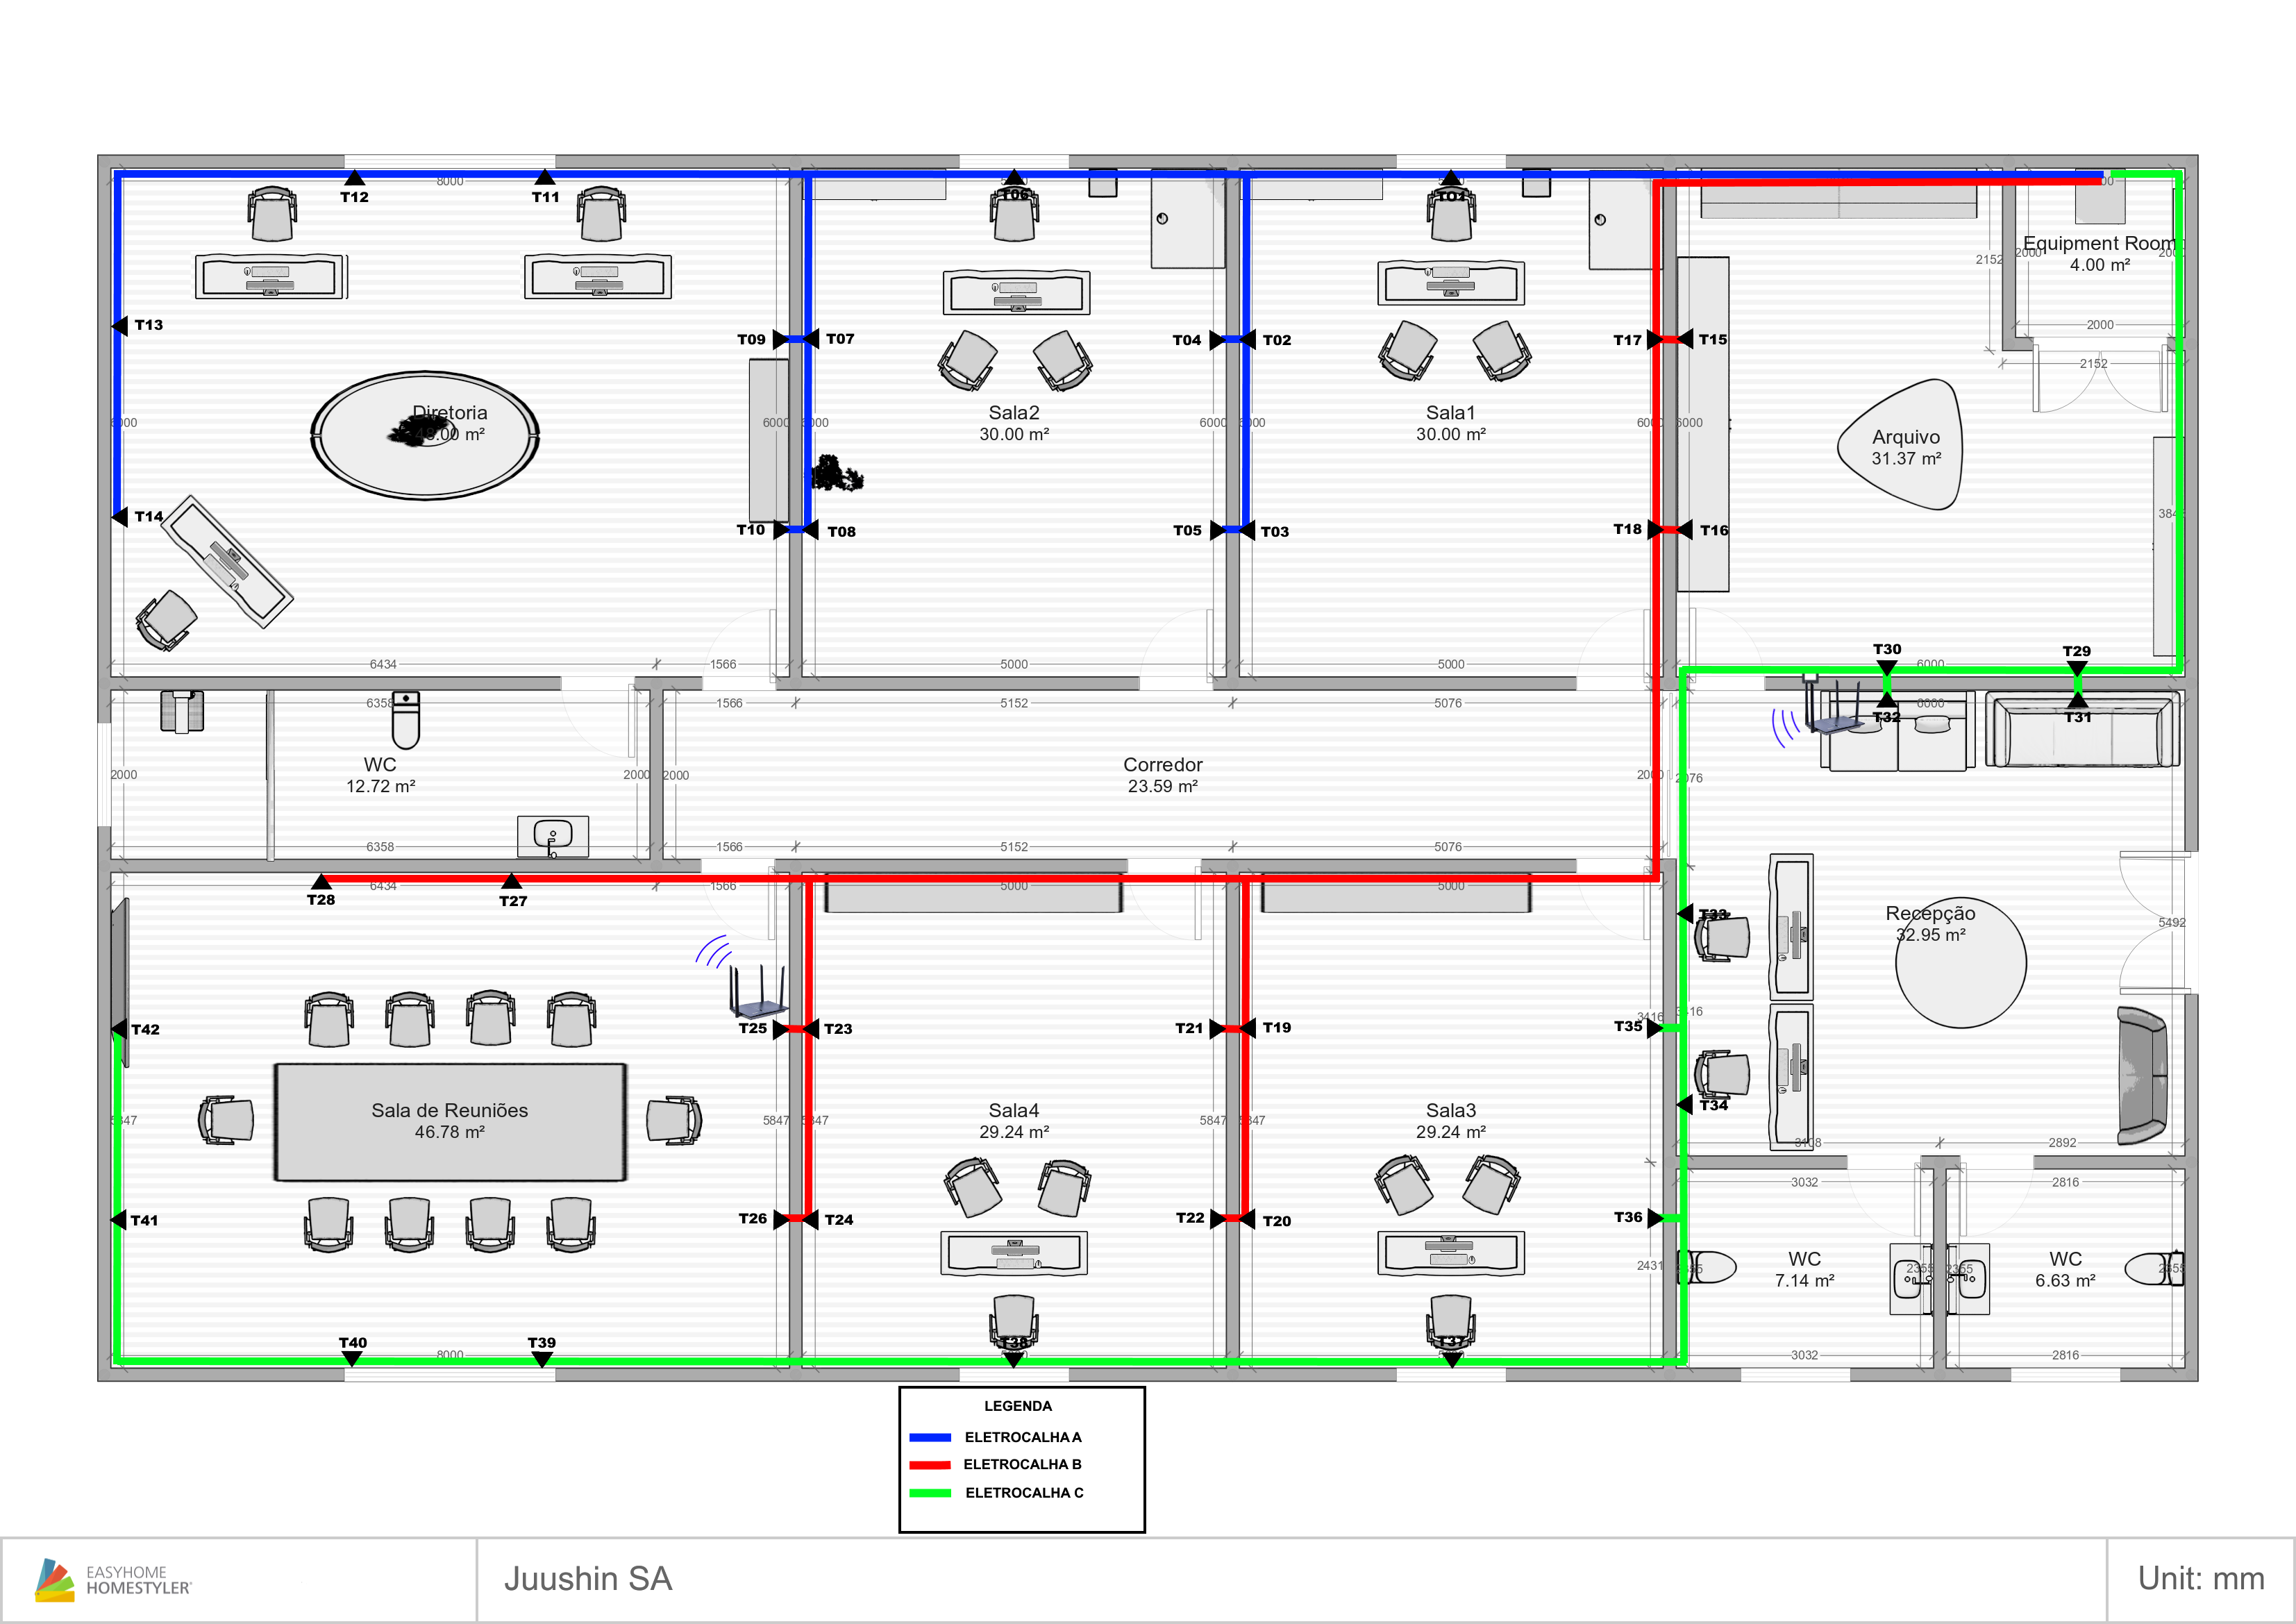
\includegraphics[width=\textwidth]{fig3}
		}
		\caption{Encaminhamento}
		\label{fig3}
	\end{figure}
	
	%Retornar ao formato A4
	\clearpage
	\KOMAoptions{paper=a4, paper=portrait, DIV=calc}
	\recalctypearea
	%-- reinicio em A4 
	\subsection{Memorial descritivo}
	
\begin{table}[h!]
	\centering
	\caption{Componentes Utilizados}
	\label{tab2} %com este label vc faz referencia no texto
	\begin{tabular}{|l|l|l|}
		\hline
		Componentes                                   & Quantidade & Fabricante      \\ \hline
		Abraçadeira Nylon 2,5 x 100mm c/100			       & 5          & Western         \\ \hline
		Cabo De Rede Furukawa Cat6 U/utp 305m     		   & 3          & Furukawa        \\ \hline
		Kit 10U Cx+tampa + 1 Tomada Rj45 Cat6              & 5          & Tramontina      \\ \hline
		Patch Cord Cat6 1,5m Gigalan Furukawa              & 50         & Furukawa        \\ \hline
		Patch Cord Cat6 2,5m Gigalan Furukawa              & 20         & Furukawa        \\ \hline
		Patch Panel Cat.6 48 Posições                      & 1          & Itcomtech        \\ \hline
		Rack 44 U                                          & 1          & CWB Metal		  \\ \hline
		Régua tomadas Com 12 Tomadas Bivolt 			   & 1          & Ipec            \\ \hline
		Switch 48 portas                                   & 1          & HP              \\ \hline
	\end{tabular}
\end{table}
	
	\subsection{Identificação dos cabos}

	De acordo com a norma ANSI/EIA/TIA - 606, cada unidade de terminação deve ter uma identificação exclusiva, conforme a norma ANSI/EIA/TIA - 606. Deste modo a identificação dos cabos seguirá o seguinte padrão:
	
	\subitem Txx - Ponto de comunicação
	\subitem W - Calha
	\subitem Pxx - Porta do Patch Panel
	\subitem Y - UTP(U), STP(S), FIBRA OTICA (Fo)
	\subitem Cxx - Número do cabo
	
	
    \textbf{Exemplo:} 
    
	\begin{figure}[h]
		\centering
		
		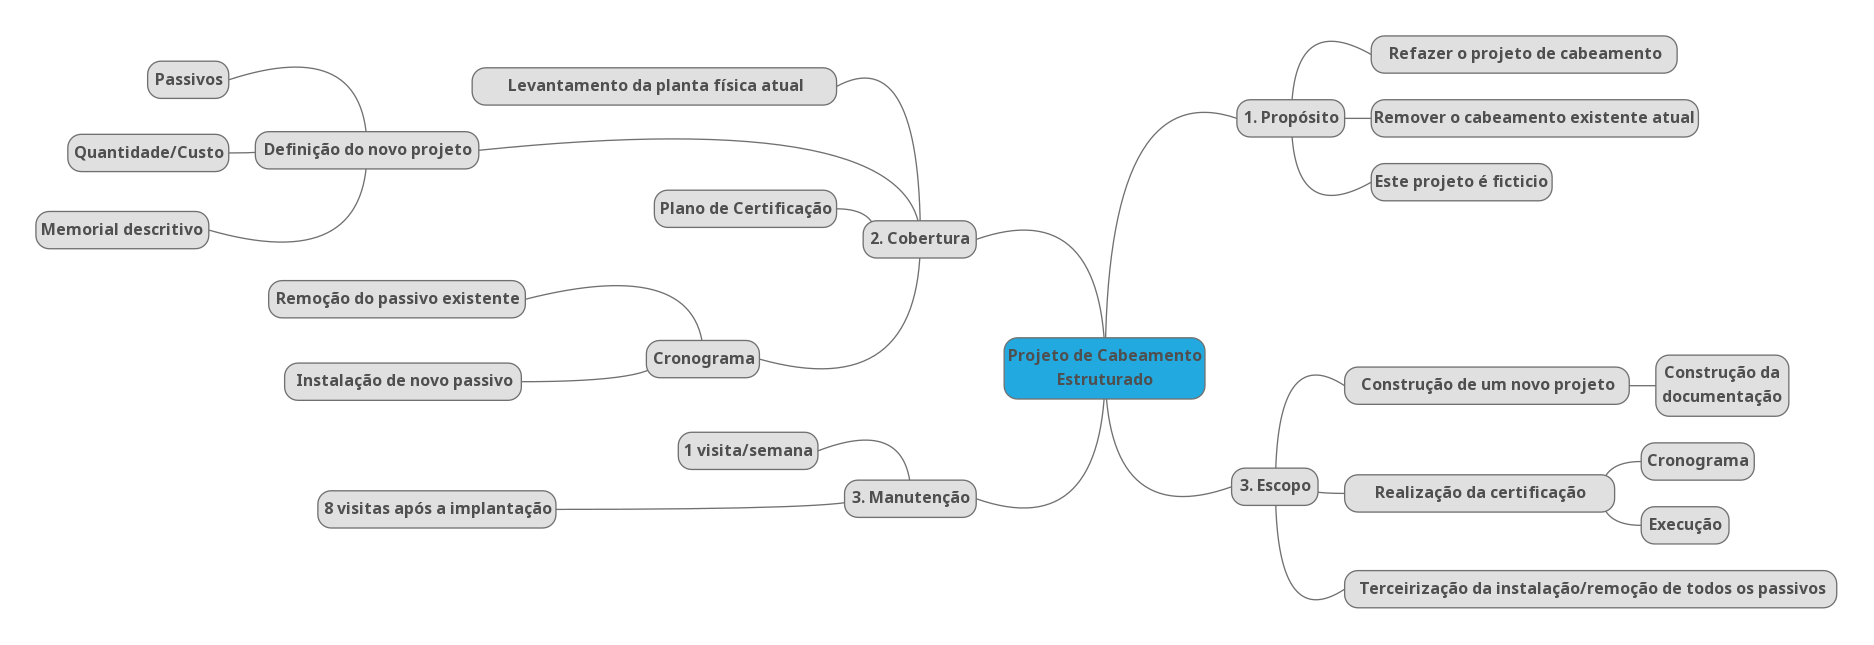
\includegraphics[width=4cm]{fig4}
		\caption{Identificação de Cabo}
		\label{fig4}
	\end{figure}
	A figura \ref{fig4} indica o cabo 01, que liga a porta 1 do Patch Panel ao Ponto de Telecomunicações 01, passando pela calha A no primeiro Andar. O tipo de cabo usado é UTP.
\clearpage	
\begin{table}[h]\footnotesize
	\centering
	\caption{Pontos}	
	\label{tab3} %com este label vc faz referencia no texto
		\begin{tabular}{|l|l|l|l|l|}
			\hline
			PONTO DE COMUNICAÇÃO & CALHA & PORTA & Nº CABO & DIST (M)    \\ \hline
			T01                 & A     & 1                 & 001      & 8           \\ \hline
			T02                 & A     & 2                 & 002      & 12,5 \\ \hline
			T03                 & A     & 3                 & 003      & 14,5 \\ \hline
			T04                 & A     & 4                 & 004      & 13   \\ \hline
			T05                 & A     & 5                 & 005      & 15    \\ \hline
			T06                 & A     & 6                 & 006      & 13    \\ \hline
			T07                 & A     & 7                 & 007      & 17,5 \\ \hline
			T08                 & A     & 8                 & 008      & 19,5 \\ \hline
			T09                 & A     & 9                 & 009      & 18           \\ \hline
			T10                 & A     & 10                & 010      & 20           \\ \hline
			T11                 & A     & 11                & 011      & 18           \\ \hline
			T12                 & A     & 12                & 012      & 21           \\ \hline
			T13                 & A     & 13                & 013      & 25,5 \\ \hline
			T14                 & A     & 14                & 014      & 27,5 \\ \hline
			T15                 & B     & 15                & 015      & 8            \\ \hline
			T16                 & B     & 16                & 016      & 10           \\ \hline
			T17                 & B     & 17                & 017      & 7,5 \\ \hline
			T18                 & B     & 18                & 018      & 9,5 \\ \hline
			T19                 & B     & 19                & 019      & 20,5 \\ \hline
			T20                 & B     & 20                & 020      & 22,5 \\ \hline
			T21                 & B     & 21                & 021      & 21   \\ \hline
			T22                 & B     & 22                & 022      & 23    \\ \hline
			T23                 & B     & 23                & 023      & 25,5 \\ \hline
			T24                 & B     & 24                & 024      & 27,5 \\ \hline
			T25                 & B     & 25                & 025      & 26   \\ \hline
			T26                 & B     & 26                & 026      & 28  \\ \hline
			T27                 & B     & 27                & 027      & 26,5 \\ \hline
			T28                 & B     & 28                & 028      & 29  \\ \hline
			T29                 & C     & 29                & 029      & 8   \\ \hline
			T30                 & C     & 30                & 030      & 10  \\ \hline
			T31                 & C     & 31                & 031      & 8,5 \\ \hline
			T32                 & C     & 32                & 032      & 10,5 \\ \hline
			T33                 & C     & 33                & 033      & 15,5 \\ \hline
			T34                 & C     & 34                & 034      & 16,5 \\ \hline
			T35                 & C     & 35                & 035      & 15   \\ \hline
			T36                 & C     & 36                & 036      & 17  \\ \hline
			T37                 & C     & 37                & 037      & 22  \\ \hline
			T38                 & C     & 38                & 038      & 27,5 \\ \hline
			T39                 & C     & 39                & 039      & 32,5 \\ \hline
			T40                 & C     & 40                & 040      & 35   \\ \hline
			T41                 & C     & 41                & 041      & 39,5 \\ \hline
			T42                 & C     & 42                & 042      & 41,5 \\ \hline
		\end{tabular}
	\end{table}
\clearpage	
	
	\section{Implantação}
A figura \ref{fig5} apresenta tabela com o cronograma de implantação previsto. O cronograma já engloba eventuais atrasos, contudo a implantação deve ocorrer dentro de 4 semanas.
		\begin{figure}[h]
			\centering
			
			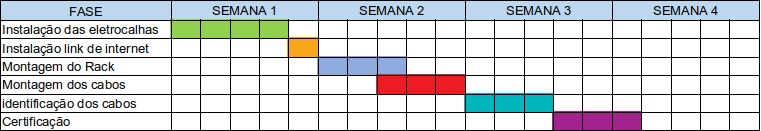
\includegraphics[width=\textwidth]{fig5}
			\caption{Cronograma de implantação}
			\label{fig5}
		\end{figure}
	
	\section{Plano de certificação}
	Quais seriam as etapas para a certificação? 
	Quais os locais e horários para execução da certificação na rede? Toda rede será certificada?
	Como os testes seriam executados?
	Quais relatórios de certificação serão (ou deveriam ser) entregues? 
	
	\section{Plano de manutenção}
	
	Revisões periódicas na rede, emissão de certificados para novos pontos.
	
	\subsection{Plano de expansão}
	A empresa acaba de passar por um processo de expansão, mas tem se preparado para crescimentos futuros, por isso o projeto de rede atual já conta com pontos de comunicação sobressalentes e a própria estrutura predial já prevê uma possível ampliação para até 3 andares. A sala de equipamentos está localizada em um ponto onde será possível a criação de um backbone para esta  ampliação, sendo recomendado o uso de fibra ótica para este fim. O Rack atual já tem espaço para instalação de novos equipamentos que atendam a demanda futura.
	
	\section{Risco}
	A estrutura de rede em si não apresenta grandes riscos, uma vez que os cabos de rede passam sob o piso elevado, devidamente acondicionados dentro de eletrocalhas e longe do cabeamento elétrico. A sala de Equipamentos possui portas com trancas assim como o Rack onde ficarão os equipamentos, impedindo assim o acesso não autorizado. A sala de equipamentos possui refrigeração, pois está localizada dentro da sala de Arquivos, que possui também sistema de combate a incendios. A parte elétrica conta ainda com protetores de surto e o aterramento dos equipamentos de rede é separado do aterramento do prédio em si.
	
	\section{Orçamento}
	\begin{table}[h!]\footnotesize
			\centering
		\caption{Custos do Projeto}
		\label{tab3} %com este label vc faz referencia no texto
	%	\begin{center}
		\renewcommand{\arraystretch}{1.5}
		\begin{tabular}{|l|l|l|l|}
			\hline
			Componente                                        & Fabricante      & Preço        & Total         \\ \hline
			Abraçadeira Nylon 2,5 x 100mm c/100 Branca        & Western         & R\$ 1,83     & R\$ 9,15      \\ \hline
			Cabo De Rede Furukawa Sohoplus Cat6 U/utp 305m    & Furukawa        & R\$ 590,00   & R\$ 1.770,00  \\ \hline
			Kit 10 Uni Cj Cx+tampa + 1 Tomada Rj 45 Cat.6     & Tramontina      & R\$ 144,28   & R\$ 721,40    \\ \hline
			Patch Cord Cat6 1,5m Gigalan Furukawa vermelho    & Furukawa        & R\$ 26,90    & R\$ 1.345,00  \\ \hline
			Patch Cord Cat6 2,5m Gigalan Furukawa vermelho    & Furukawa        & R\$ 37,90    & R\$ 758,00    \\ \hline
			Patch Panel Cat.6 24 Posicoes                     & Furukawa        & R\$ 599,99   & R\$ 1.199,98  \\ \hline
			Rack 44 U                                         & Mundo dos Racks & R\$ 1.673,76 & R\$ 1.673,76  \\ \hline
			Régua tomadasRegua Rack 19" Com 12 Tomadas Bivolt & Ipec            & R\$ 33,90    & R\$ 33,90     \\ \hline
			Switch 48 portas                                  & HP              & R\$ 2.535,90 & R\$ 2.535,90  \\ \hline
			Eletrocalha 50x50 3m                              & Prime Metal     & R\$ 33,21    & R\$ 2.092,23  \\ \hline
			Eletrocalha Curva Horiz 90 50x50                  & Prime Metal     & R\$ 18,15    & R\$ 145,2     \\ \hline
			Eletrocalha Te 90 50x50                           & Prime Metal     & R\$ 23,48    & R\$ 93,92     \\ \hline
			Eletroduto Em Pvc c/ 3 Metros                     & Tigre           & R\$ 12,99    & R\$ 90,93     \\ \hline
			\multicolumn{3}{|l|}{TOTAL GERAL}                                                  & R\$ 12.469,37 \\ \hline
		\end{tabular}
%	\end{center}
	\end{table}
	
	\section{Recomendações}
	Observações e recomendações para o cliente.
	
	\section{Referências bibliográficas}
	Utilize o mendley, o jabref ou diretamente o bibtex para gerenciar suas referências biliográficas. As referências são criadas automaticamente de acordo com o uso no texto.
	
	Exemplo: Redes de computadores, segundo \cite{t2013} é considerada..... Já \cite{kurose2010} apresenta uma versão...
	
	Analisando os pressupostos de \cite{ref3} e \cite{ref4} concluimos que....
	
	
	\renewcommand\refname{} %%Referências bibliográficas}  
	\bibliographystyle{ieeetr}
	\bibliography{referencias}  

\end{document}	
